% !TEX root = ../main.tex
\subsection{FMT Efficiency}
    % TODO. Explain 3 sources of low efficiency.

    % Low FMT efficiency + list sources.
    Compared to the alignment work described in section \ref{sec::fmtalignmentandreconstruction}, a low FMT is observed in this analysis.
    This can be seen in figure \ref{fig::vz_012933}.
    Upon inspection, three causes can be blamed for this: the application of incorrect alignment constants, a general FMT offline reconstruction issue, and the geometry effect described in section \ref{ssec::validationandresults}.

    \begin{figure}[b!]
        \centering\frame{
        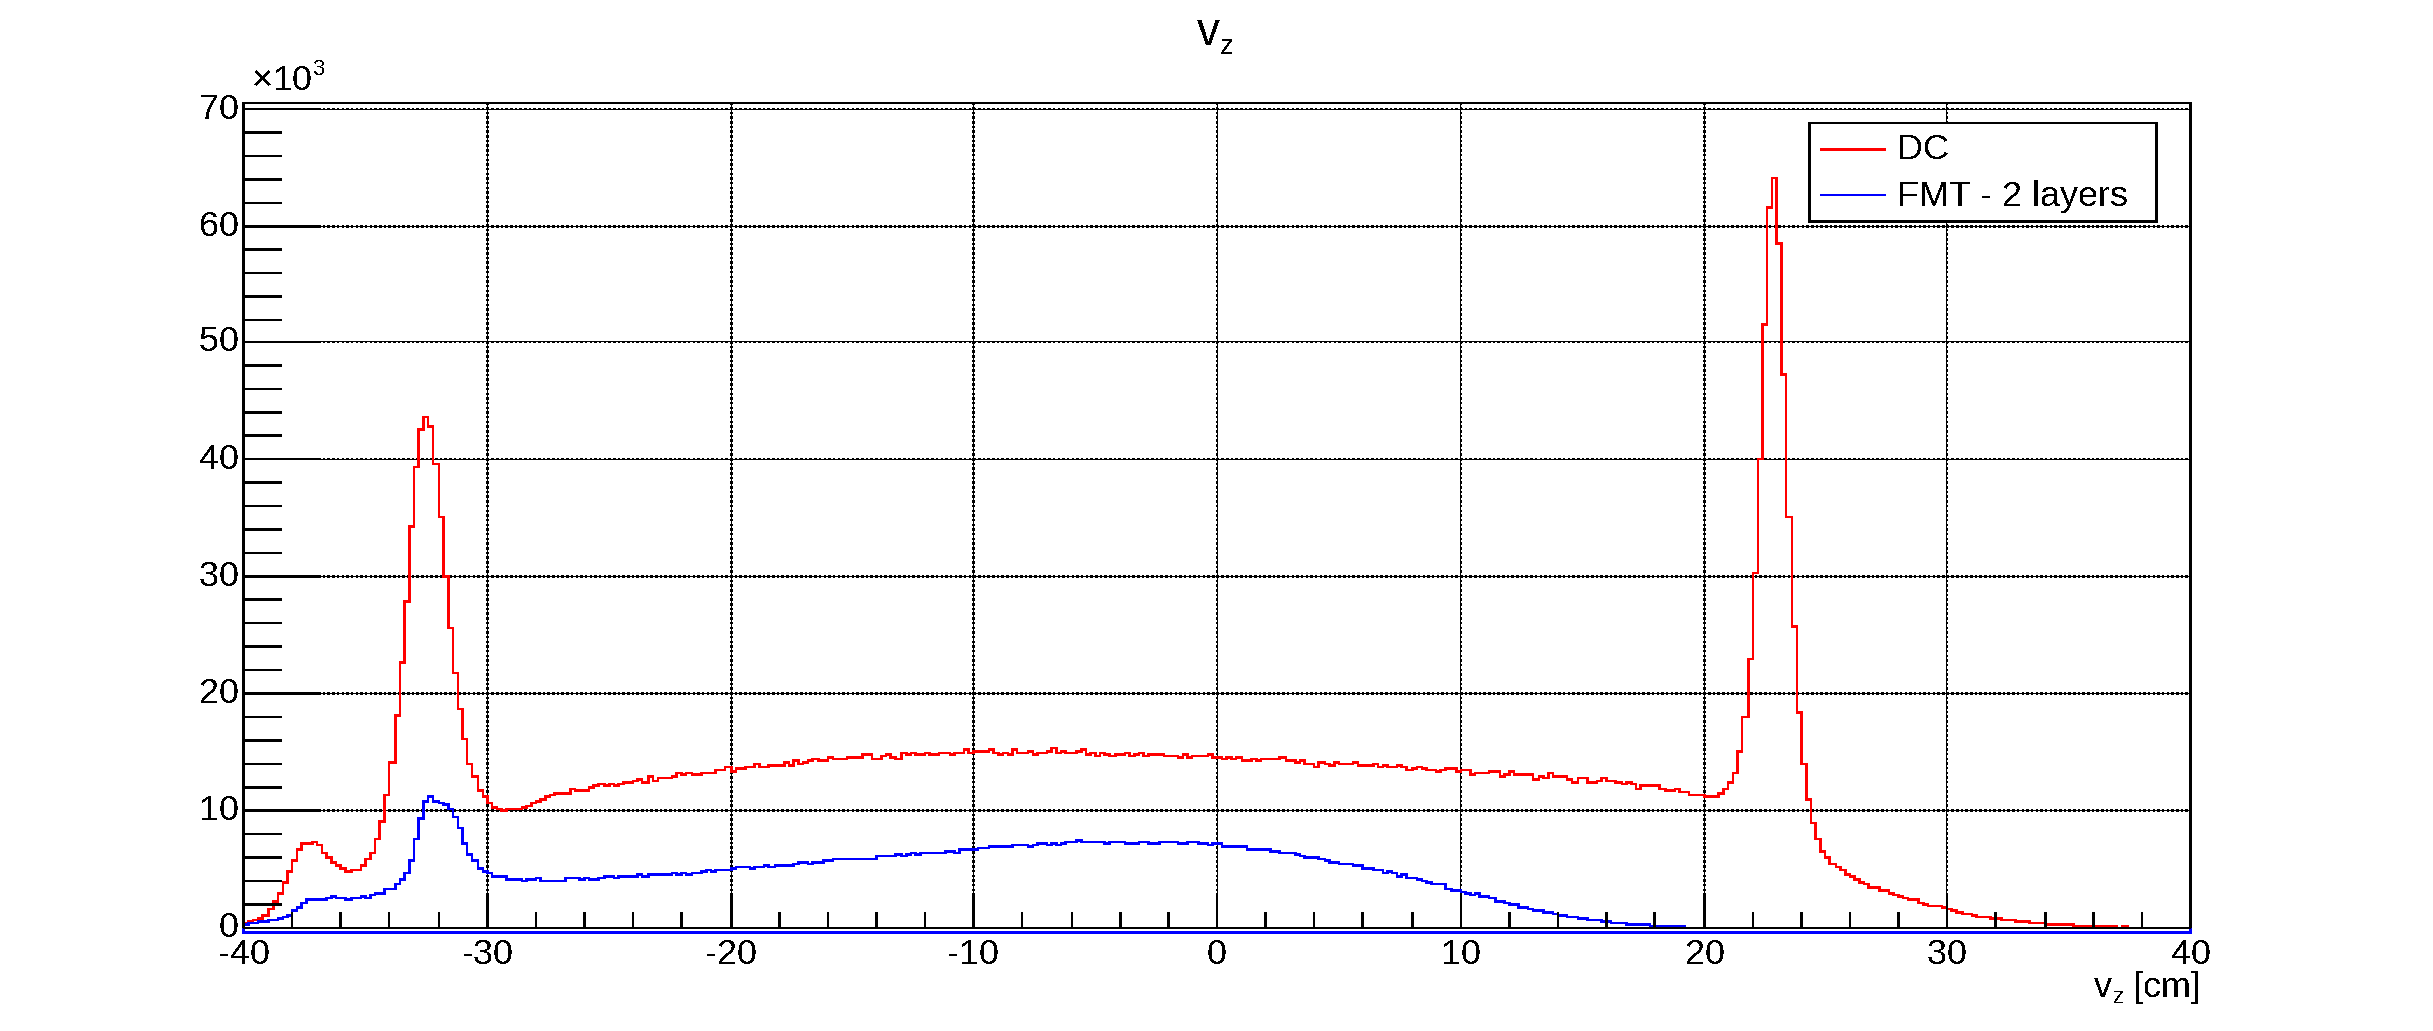
\includegraphics[width=\textwidth]{14resultsandconclusions/img/10vz_012933.pdf}}
        \caption[$v_z$ for DC and FMT, run 12933]{$v_z$ for DC (in red) and FMT (in blue). Summer 2020 data, run 12933. The wide peaks in FMT suggest an uncorrected misalignment.}
        \label{fig::vz_012933}
    \end{figure}

% --+ Alignment Effect +--------------------------------------------------------
    \subsubsection{Alignment Effect}
        % Introduction: The problem.
        The RG-F experiment's data is divided based on the season over which runs take place, thus there is Spring 2020 and Summer 2020 data.
        Based on the run group's guidelines, it is recommended to use Summer data, as it has seen more calibration than the Spring data.
        However, this calibration work hasn't included the FMT detector, and a strong misalignment effect is observed.

        % Cause of the problem.
        By simple visual inspection, two peaks can be clearly seen between $z = -36$ cm and $z = -30$ cm in figure \ref{fig::dc_vs_fmt_vz_011983}.
        These peaks are merged in figure \ref{fig::vz_012933}.
        As discussed in section \ref{sec::fmtalignmentandreconstruction}, this issue comes from a lack of correction for FMT misalignemnts.

        % Solution.
        The simplest solution is to use Spring data.
        While more work has been put on Summer data, it mainly pertains to the central detector; unrelated to this analysis.
        Figure \ref{fig::vz_012016} shows the same $v_z$ plot from Spring 2020 run 12016.
        Both peaks are clearly visible in this plot, suggesting that misalignments are properly accounted for in the run.

        \begin{figure}[b!]
            \centering\frame{
            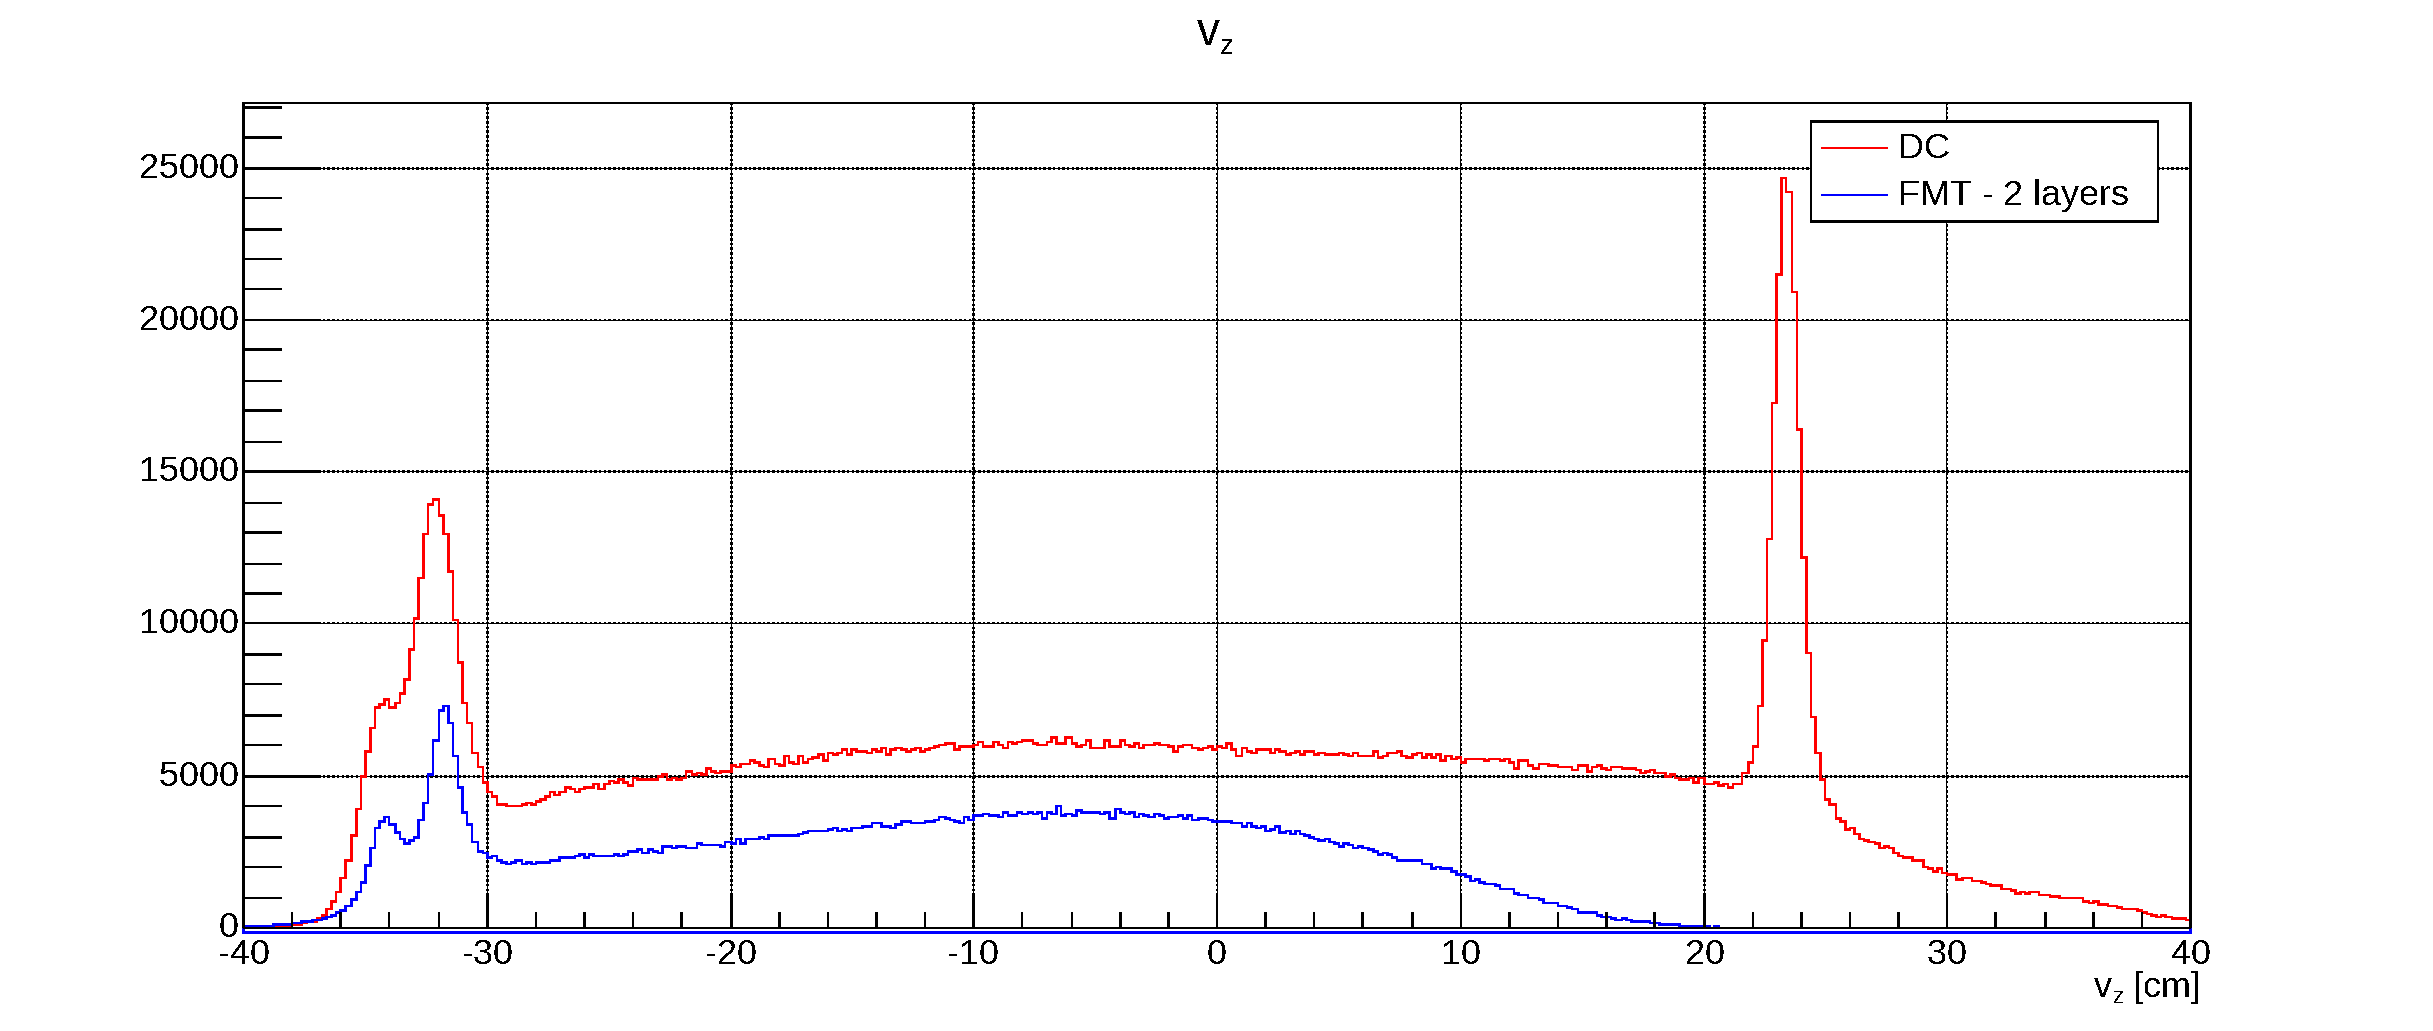
\includegraphics[width=\textwidth]{14resultsandconclusions/img/10vz_012016.pdf}}
            \caption[$v_z$ for DC and FMT, run 12016]{$v_z$ for DC (in red) and FMT (in blue). Spring 2020 data, run 12016. The upstream twin peaks can be clearly distinguished, suggesting a correct misalignment correction.}
            \label{fig::vz_012016}
        \end{figure}

    % TODO. Reconstruction effect.

    % TODO. Geometry effect.

    % TODO. Add FMT efficiency study w/ and w/out geometry cut.
